\documentclass[titlepage]{article}
\usepackage[margin=2.5cm]{geometry}
\usepackage{enumerate}
\usepackage{fancyhdr}
\usepackage{graphicx}
\usepackage{amsmath}
\usepackage{tikz}
\usepackage{csvsimple}
\usepackage{pgfplots}

\pagestyle{fancy}
\fancyhead{}
\fancyfoot{}
\rfoot{\thepage}

\usepackage{float}
\usepackage{listings, color, times, textcomp, float, hyperref, subfigure}
\definecolor{mygreen}{RGB}{28,172,0} % color values Red, Green, Blue
\definecolor{mylilas}{RGB}{170,55,241}
\lstset{language=Matlab, basicstyle=\scriptsize\ttfamily,breaklines=true,frame=single,morekeywords={matlab2tikz},
keywordstyle=\color{blue}, morekeywords=[2]{1}, keywordstyle=[2]{\color{black}}, identifierstyle=\color{black},
stringstyle=\color{mylilas}, commentstyle=\color{mygreen}, showstringspaces=false, numbers=left,
numberstyle={\tiny \color{black}}, numbersep=9pt, emph=[1]{for,end,break},emphstyle=[1]\color{red},
literate={~} {\texttildelow}{1}}

\newcommand{\exo}[1]{\section*{Exercise #1}}
\newcommand{\prob}[1]{\section*{Problem #1}}
\newcommand{\quest}[1]{\section*{Question #1}}
\newcommand{\e}{&=}
\newcommand{\p}[1]{\times 10^{#1}}
\renewcommand{\headrulewidth}{0pt}
\renewcommand{\footrulewidth}{0.5pt}

\DeclareMathOperator\erf{erf}

\title{Effective Vaccination Strategies for an H1N1 Epidemic in Ithaca, New York}
\author{Prepared by Paul Chesnais (pmc85), Christopher Silvia (cps232), \\ and Ryan Vogan (rcv39) in completion of Project 01 for MATH 3610}
\date{September 30, 2015}

\begin{document}
\maketitle
\thispagestyle{fancy}

\section{Introduction}
	For this project, we were tasked with modeling a H1N1 outbreak in Ithaca, New York. The goal of this effort was to provide local government officials with a recommended plan for distributing 4000 vaccines among the city's approximately 60000 inhabitants. The strategies that officials are particularly interested in are:
	\begin{itemize}
		\item[1.]
			Focus vaccination efforts on more connected individuals
		\item[2.]
			Focus vaccination efforts on more frail or susceptible individuals
	\end{itemize}
	They wanted to know which strategy would be better under two possible scenarios:
	\begin{itemize}
		\item[1.]
			An outbreak of the H1N1 virus
		\item[2.]
			An outbreak of a new H1N1 strain that is twenty times as deadly
	\end{itemize}
	When evaluating possible strategies, we considered the following two metrics:
	\begin{itemize}
		\item[1.]
			Total number of deaths
		\item[2.]
			Total number of person-months of infection
	\end{itemize}
	Therefore, a particular distribution of vaccines is considered better if it saves more lives and prevents more suffering. 

\section{Deterministic SIR Model}
\subsection{Algorithm and Assumptions}
	Our initial research on epidemiology discovered a common model known as the SIR approach \cite{SIR}. In this model, the population is segmented into three compartments that represent susceptible, infected, and removed states. This model assumes:
	\begin{itemize}
		\item[1.]
			A constant population size $N$
		\item[2.]
			Constant rates of transmission and recovery
		\item[3.]
			No births or deaths
		\item[4.]
			A well-mixed population
	\end{itemize}
	Define $S$ to be the number of susceptible individuals, $I$ to be the number of infected individuals, $R$ to be the number of recovered individuals, and $N$ to be the total population of Ithaca. Now normalize these variables  to consider the fraction of the total population in each compartment, such that $s = S/N$, $i = I/N$, $r = R/N$. Then the model is governed by the following three ordinary differential equations \cite{SIR}:
	\[
		\frac{ds}{dt} = - \beta s i
	\]
	\[
		\frac{di}{dt} = \beta s i - \gamma i
	\]
	\[
		\frac{dr}{dt} = \gamma i
	\]
	Here $\beta$ represents the effective contact rate, and $\gamma$ is the recovery rate \cite{SIR}. It is important to note that in this variant of the SIR model, we interpreted R to stand for Recovered rather than removed. Traditionally, the removed state represents all individuals who are not infected and are incapable of becoming infected again. This encompasses both individuals who recovered and those who died. We chose to separate mortality rates out of the removal rate so that this parameter could be adjusted for the deadlier virus strain. Then the system of equations becomes:
	\[
		\frac{ds}{dt} = - \beta s i
	\]
	\[
		\frac{di}{dt} =  i (\beta s -\gamma - \mu)
	\]
	\[
		\frac{dr}{dt} = \gamma i
	\]
	\[
		\frac{d\delta}{dt} = \mu i
	\]
	Here, $\mu$ is the death rate, and $\delta$ is the fraction of the population that has died from the swine flu. Therefore, this adds a fourth compartment, where a sick person can either recover or die. The final parameter necessary to model vaccination strategies on a homogeneous population is the vaccination rate itself. When this is added, the system becomes\cite{applet}:
	\[
		\frac{ds}{dt} = - \beta s i - \nu
	\]
	\[
		\frac{di}{dt} =  i (\beta s -\gamma - \mu)
	\]
	\[
		\frac{dr}{dt} = \gamma i + \nu
	\]
	\[
		\frac{d\delta}{dt} = \mu i
	\]
	Where $\nu$ is the fraction of the total population that gets vaccinated in a single month. This does not depend on the fractions of susceptible or infected individuals because we have a constant $4000$ vaccines per month. In the actual implementation of this model, it was necessary to code in a conditional statement that set this constant to $0$ once the susceptible population completely diminished, otherwise this would result in negative population values for that compartment. Also, note that this assumes that the number of vaccines distributed grows linearly throughout the month, finally reaching $4000$ at the very end.\\ 

	The final missing piece of this model was to do away with the well-mixed assumption. This was crucial for us to make the distinction between highly-connected and frail individuals as requested by the government officials. We decided to segment the population into four categories. They are babies/toddlers ($<$ 4 years old), children/teens (between 5 and 24 years old), adults (between 25 and 65 years old), and seniors ($>$ 65 years old). These categorizations were chosen based on evidence for mortality rates that will be discussed in the ``Parameter Justifications'' section. This effectively quadruples our number of compartments, where the final set of ODE's is then:
	\[
		\frac{ds_k}{dt} = - (\beta_{k,1} i_1 + \beta_{k,2} i_2 + \beta_{k,3} i_3 + \beta_{k,4} i_4) s_k - \nu_k
	\]
	\[
		\frac{di_k}{dt} =  (\beta_{k,1} i_1 + \beta_{k,2} i_2 + \beta_{k,3} i_3 + \beta_{k,4} i_4) s_k - i_k (\gamma + \mu_k)
	\]
	\[
		\frac{dr_k}{dt} = \gamma i_k + \nu_k
	\]
	\[
		\frac{d\delta_k}{dt} = \mu_k i_k
	\]
	Here, the subscript k indicates that the parameter belongs to the kth segment of the population, where k = 1 for babies/toddlers, k = 2 for children/teens, k=3 for adults, and k=4 for seniors. $\beta_{i,j}$ represents the rate of contact of an individual of type $i$ from an individual of type $j$. The values of these parameters come from a matrix called the Next-Generation Matrix \cite{NGM} that will be discussed in the ``Parameter Justifications'' section. Finally, note that there is no subscript on the $\gamma$ parameter, meaning we assume the recovery rate to be constant for all four age group. This is because recovery rate is related to the duration of an infection, as will be discussed in ``Parameter Justifications''.\\

	We used MATLAB's built in ode45 solver on this system of equations to compute the fractions of susceptible, infected, recovered, and dead individuals for each sub-segment of the population over time.
\subsection{Parameter Justifications}
	An important dependent parameter for modeling epidemics is known as the Basic Reproduction rate \cite{SIR}. This quantity is:
	\[
		R_0 = r c d
	\]
	Where $r$ is the probability of an infection given contact between a susceptible and infected individual, $c$ is the average rate of contact between susceptible and infected individuals, and $d$ is the duration of infectiousness \cite{SIR}. This $R_0$ value can be used to compute our $\beta$ value in the SIR model. Because we need the number of infected individuals to increase for the basic SIR model, we have:
	\[
		\frac{di}{dt} = \beta s i - \gamma i > 0
	\]
	\[
		\frac{\beta s i}{\gamma} > i
	\]
	\begin{center}
		$s \approx 1$ at the start of the epidemic
	\end{center}
	\[
		\frac{\beta}{\gamma} = R_0 > 1
	\]
	This is then the relationship between $\beta$ and $R_0$ \cite{SIR}. We can compute $\gamma$ if we define it to be $1/d$, the duration of infectiousness \cite{SIR}. The fact that we assume this duration of infectiousness to be the same across all ages is why we see a constant recovery rate $\gamma$.The average duration of infectiousness for swine flu is one week \cite{oneweek}(.25 months), and the Basic Reproduction Number is 1.5 \cite{R0}, so we have $\gamma = 4$ and $\beta = 6$ in the standard SIR model. When data was first being collected in the 2009 outbreak of the swine flu, approximately 7\% of the population was infected \cite{init}, so we began our SIR model at s = .95 and r = .05. Finally, in order to set the death rate for the homogeneous SIR model, we discovered that of approximately 60.8 million infections in 2009, 12,469 resulted in deaths \cite{deathpercent}. Dividing this fraction between 12 months leads to $\mu = 0.00001709$

    For the more complicated SIR model, however, single parameter values do not work because we have four distinct sub-populations. These sub-populations were chosen based on the following bar chart:

	\begin{figure}[h!]
	\centering
		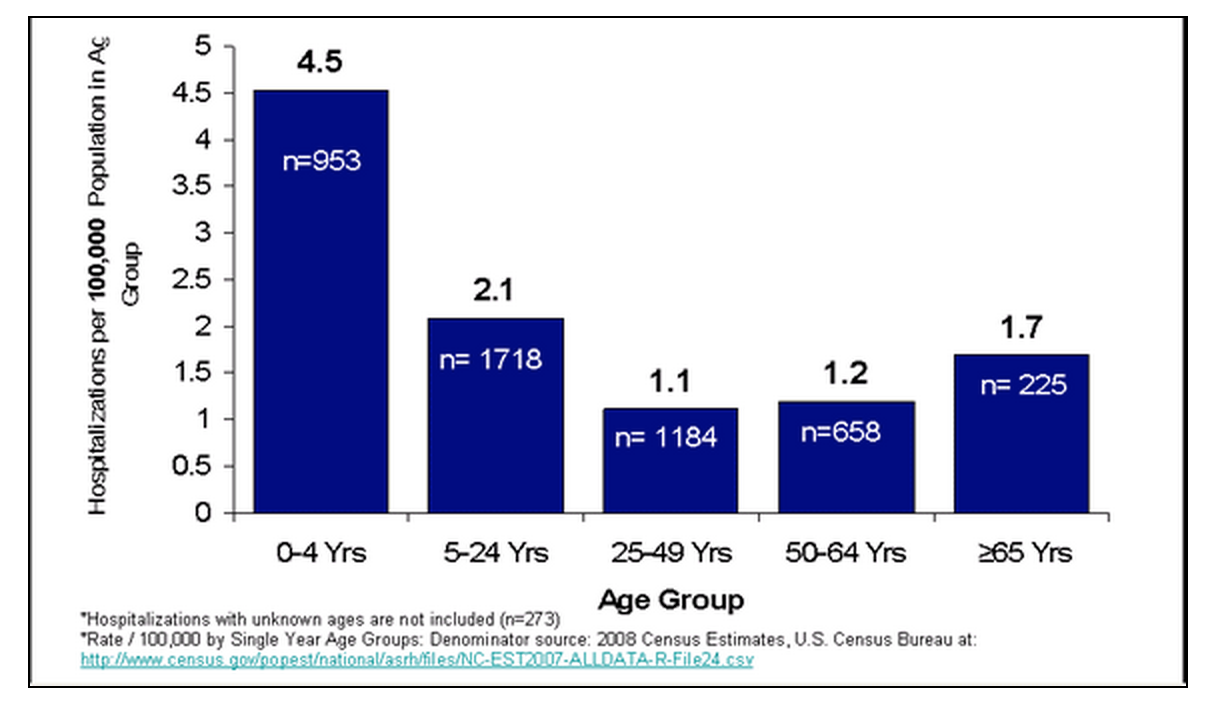
\includegraphics[width=.5\textwidth]{figures/death_graph.png}
        \caption{Mortality rates by age group \cite{deathgraph}}
	\end{figure}

    Here you can see that the death rate is relatively constant from age 25-64, so we grouped these ranges together into the ``adults'' category. The $\mu$ value for each sub-population was simply these numbers scaled by the global $\mu$ found above. The fractions of the total population that each of these sub-groups occupied \cite{pop} was found to be (.0248, .6058, 3066, .0628). Finally, the single $\beta$ had to be derived from a Next Generation Matrix. This is an equivalent of the $B0$ value for multiple sub-populations with transitions between each. This is defined to be that the jth column represents the average number of infections of individuals of type i from an individual of type j \cite{SIR}. These values were largely hand-picked for the 4 sub-population model, but we tried not to deviate too far from 1.5.
    \[
        R0 = 
        \begin{bmatrix}
        3.00 & 0.10 & 0.10 & 0.10 \\
        0.10 & 3.00 & 1.00 & 0.10 \\
        2.00 & 2.00 & 1.50 & 1.00 \\
        0.10 & 0.10 & 0.50 & 1.00
        \end{bmatrix}
    \]

\subsection{Predictions}
	//TODO
% \subsection{Validation and Robustness Testing}
% 	//TODO
% \subsection{Strengths and Weaknesses}
% 	//TODO
% \subsection{Future Work}
% 	//TODO

\section{Deterministically Allocating Vaccines Between Disjoint Populations}
	Chris's stuff goes here

\section{Stochastic Model}
	Paul's stuff goes here

\section{Conclusion}
	//TODO
\section{References}
	\begin{thebibliography}{9}
	\bibitem{areconnect}
		\url{http://ithaca.areaconnect.com/statistics.htm}
	\bibitem{CIC}
		\url{http://www.cdc.gov/h1n1flu/surveillanceqa.htm}
	\bibitem{walph}
		Wolfram Research Inc.,
		\emph{WolframAlpha},
		Retrieved September 26, 2015
		\url{http://www.wolframalpha.com/input/?i=ds%2Fdt+%3D+r+s+%28K+-+s+-+a+t%29}
		\url{http://www.wolframalpha.com/input/?i=%E2%88%AB+e^%28-a+x^2+%2B+b+x%29+dx}
	\bibitem{SIR}
		\url{http://web.stanford.edu/~jhj1/teachingdocs/Jones-on-R0.pdf}
	\bibitem{applet}
		\url{http://www.public.asu.edu/~hnesse/classes/sirv.html?}
	\bibitem{NGM}
		\url{http://rsif.royalsocietypublishing.org/content/7/47/873}
	\bibitem{oneweek}
		\url{https://www.cdph.ca.gov/HealthInfo/h1n1flufaqs/Pages/H1N1fluFAQs-01-GenInfo.aspx}
	\bibitem{R0}
		\url{http://www.ncbi.nlm.nih.gov/pmc/articles/PMC2715422/}
	\bibitem{deathgraph}
		\url{http://www.cdc.gov/h1n1flu/surveillanceqa.htm}
    \bibitem{init}
        \url{http://academic.udayton.edu/muhammadusman/2010Stander/H1N1.pdf}
    \bibitem{deathpercent}
        \url{http://www.cdc.gov/h1n1flu/estimates_2009_h1n1.htm}
    \bibitem{pop}
        \url{http://ithaca.areaconnect.com/statistics.htm}
	\end{thebibliography}

\section{Source Code}
	//TODO
\section{Individual Contributions}
	//TODO

\end{document}